\documentclass[../main.tex]{subfiles}

En los sistemas de posicionamiento en interiores, las``técnicas de posicionamiento'' son utilizadas para determinar y estimar la posición de un objeto.
Los sistemas de posicionamiento utilizan algoritmos que traducen las propiedades de señales recibidas a distancias y ángulos, y calculan la posición del objeto (ver Fig. \ref{fig:integracion}.). \\
A pesar de que la mayoría de técnicas, algoritmos y elementos de los sistemas de posicionamiento en interiores no son nuevos, ya que fueron implementados con anterioridad en exteriores, su comportamiento es diferente en ambos entornos. Esto ha servido de estimulo para descubrir formas de aplicar de manera óptima las técnicas de posicionamiento en la determinación de la posición.
Las dos técnicas de posicionamiento utilizadas son las \textbf{propiedades o métricas de la señal} y los \textbf{algoritmos o métodos de posicionamiento}, que se muestran en la Figura \ref{fig:tecnicas}.

\begin{figure} [h]
    \centering
    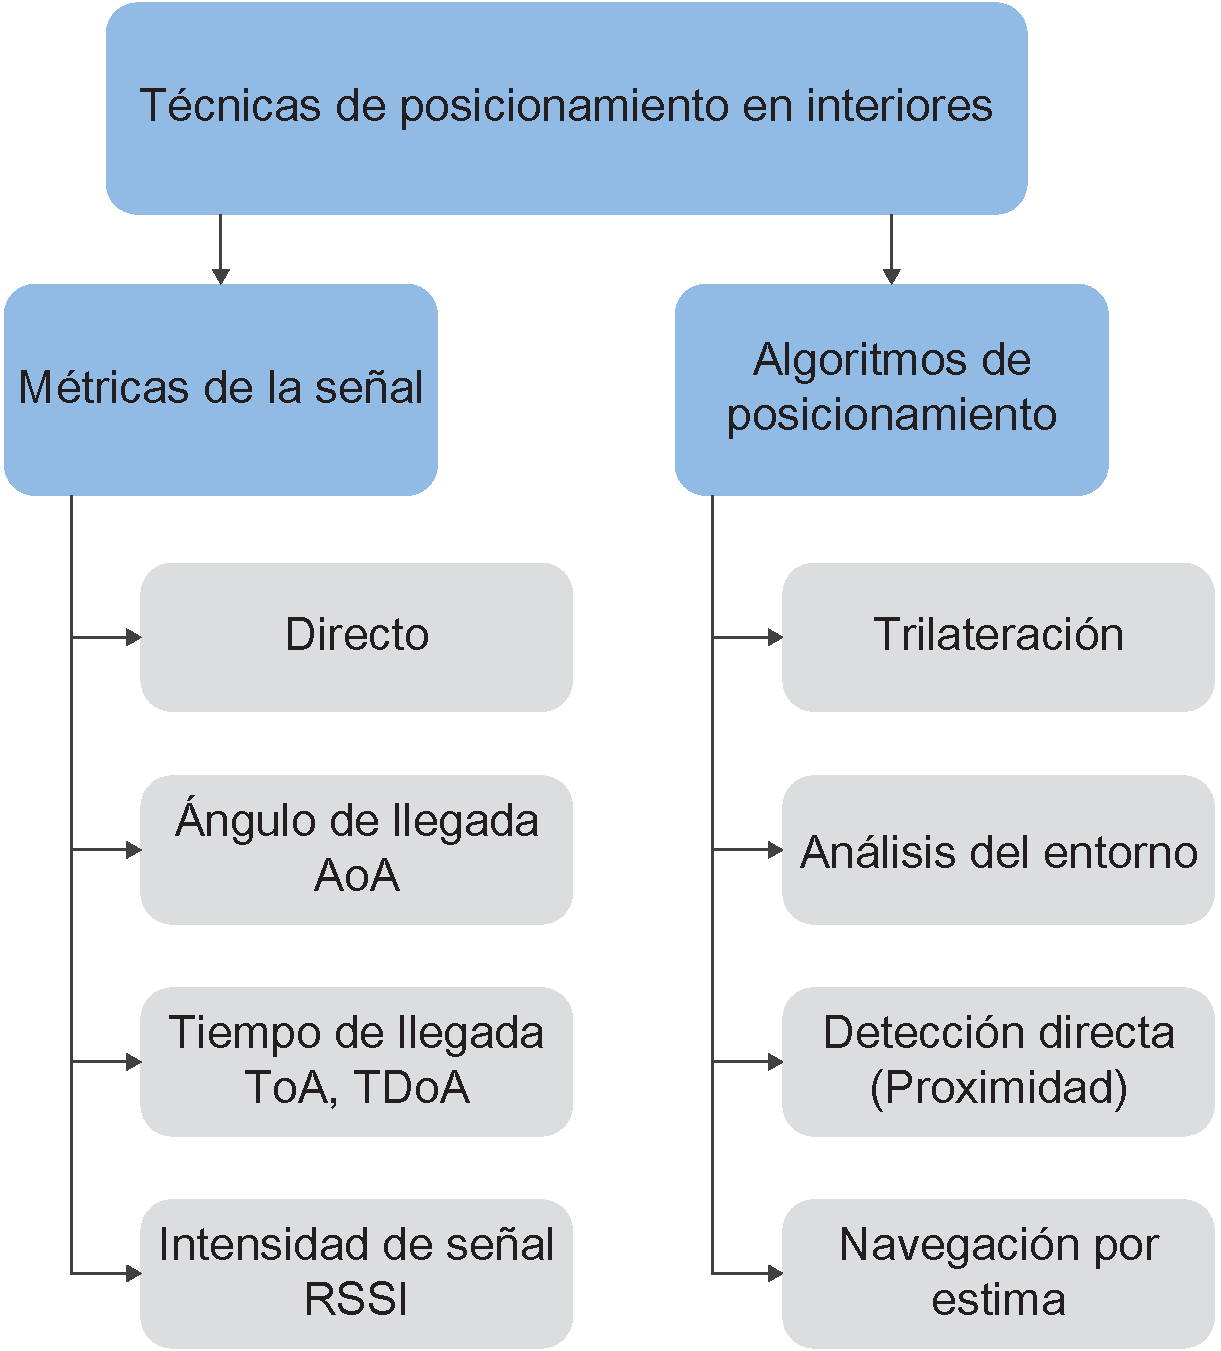
\includegraphics[width=0.6\textwidth]{tecnicas.pdf}
    \caption{Clasificación de técnicas en IPS.}
    \label{fig:tecnicas}
\end{figure}

Sin embargo, debido a que las técnicas y tecnologías de posicionamiento pueden ser de diversa índole, solo aquellas innovaciones más relevantes para el propósito de este trabajo serán expuestas y exploradas en esta sección.

\section{Métricas de la señal} \label{section:metricas}
Los sistemas de posicionamiento se pueden clasificar mediante las técnicas de medición de la señal que utilizan. Las propiedades de la señal son parámetros geométricos basados en métricas como el ángulo, la distancia o la intensidad para obtener la posición del objeto.
Existen varias técnicas de medición de la señal, pero en esta sección nos centraremos en las preponderantes: 

\begin{itemize}
    \item Medición directa o física.
    \item Ángulo de llegada (AoA, \emph{Angle of Arrival}).
    \item Tiempo de llegada (ToA, \emph{Time of Arrival}).
    \item Diferencia de tiempos de llegada (TDoA, \emph{Time Difference of Arrival}).
    \item Intensidad de señal recibida (RSSI, \emph{Received Signal Strength Indication}).
\end{itemize}

La precisión en el posicionamiento depende, en muchas ocasiones, de la precisión de la información recopilada, es decir, de la exactitud del valor de la propiedad de la señal medida. % Por ello, es necesario entender bien su funcionamiento y su medición para obtener valores precisos.

    \subsection{Medición directa} \label{subsection:directa}
    La medición directa es una técnica sencilla de obtención de distancias utilizando una acción física o movimiento, a saber: un robot que extienda una sonda hasta tocar algo sólido o que tome medidas con una cinta métrica. Las mediciones de distancia directa son fáciles de entender pero difíciles de obtener automáticamente debido a las complejidades involucradas en la coordinación del movimiento físico autónomo.

    \subsection{Ángulo de llegada} \label{subsection:aoa}
    El ángulo de llegada (AoA) proporciona una medida del ángulo en el que se recibe una señal en un dispositivo de referencia.
    El dispositivo de referencia define una línea que parte desde su posición hasta la posición donde se supone que está el objeto, con tal ángulo medido. La combinación de varias líneas de diversos dispositivos de referencia permite ubicar al objeto en la intersección de tales líneas. Al menos dos puntos de referencia ($P_1$ y $P_2$) y dos ángulos ($\theta_1$ y $\theta_2$) son necesarios para posicionar un punto en el plano (ver Figura \ref{fig:aoa}). La estimación de la posición sería la siguiente:
    
    \begin{equation}
        \begin{gathered}
            \hat{y} - y_1 = ( \hat{x} - x_1 ) \tan \theta_1 \\
            \hat{y} - y_2 = ( \hat{x} - x_2 ) \tan \theta_2
        \end{gathered}
        \label{eq:aoa_1}
    \end{equation}
    
    
    \noindent siendo $x_1$ y $y_1$ las coordenadas del punto de referencia $P_1$, $x_2$ y $y_2$ las coordenadas del punto de referencia $P_2$ y, $\hat{x}$ y $\hat{y}$ las coordenadas del punto desconocido $S$. Resolviendo las ecuaciones de \ref{eq:aoa_1}, obtendríamos la posición del punto $S (\hat{x}, \hat{y})$ \cite{Kawakami.2011}.
    
    \begin{equation}
        \left \{ 
        \begin{array}{l}{
            \hat{x} = \dfrac{x_1 \tan \theta_1 - x_2 \tan \theta_2 + y_2 - y_{1}} {\tan \theta_1 - \tan \theta_2}} \\ 
            {\hat{y} = \dfrac{\left(x_1 - x_2 \right) \tan \theta_1 \tan \theta_2 + y_2 \tan \theta_1 - \tan \theta_2}{\tan \theta_1 - y_1 \tan \theta_2}}
        \end{array}
        \right.
    \end{equation}
    
    La precisión del posicionamiento depende directamente de la calidad de la medición de los ángulos y las posiciones conocidas de los puntos de referencia. \\ La ventaja de esta técnica es que no es necesaria una sincronización en el tiempo entre las distintas referencias. Sin embargo, requiere un hardware complejo para determinar el AoA de manera precisa.
    
    \begin{figure}[h]
        \centering
        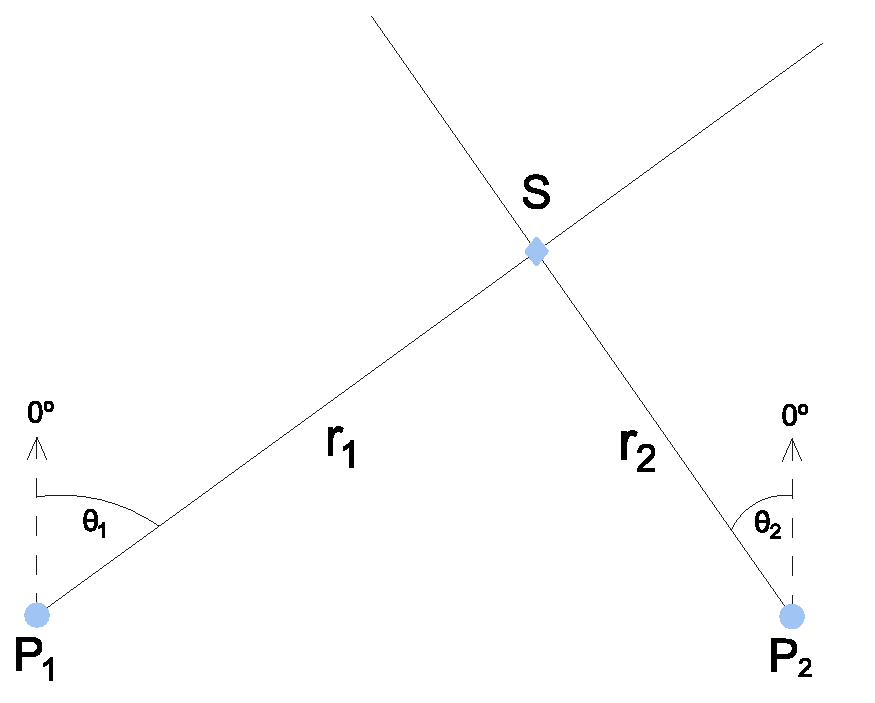
\includegraphics[width=0.5\textwidth]{aoa.pdf}
        \caption{Posicionamiento 2D basado en la medida del AoA \cite{Kawakami.2011}.}
        \label{fig:aoa}
    \end{figure}

    \subsection{Tiempo de llegada} \label{subsection:toa}
    El tiempo de llegada (ToA), también denominado tiempo de vuelo (ToF), es el tiempo que tarda la señal en ir desde el transmisor hasta el receptor. Si el receptor es capaz de obtener el ToA, $t_i$, será capaz de estimar su rango $r_i$ haciendo uso de la velocidad de la luz en el vacío $c = 3 \times 10^8 m/s$ \cite{sayed.2005} según:
    
    \begin{equation}
        r_i = c t_i
        \label{eq:rang_toa}
    \end{equation}
    
    De esta forma, con distintos dispositivos de referencia combinando sus respectivos rangos es posible determinar la posición. El ToA describe círculos alrededor de los dispositivos de referencia y aunque dos círculos son suficientes para resolver las coordenadas en el plano, se necesita un tercero para deshacerse de la ambigüedad (ver Fig. \ref{fig:toa}). \\ 
    En dos dimensiones, con $N$ referencias conocidas, $P_1$, $P_2$, ... , $P_n$, con coordenadas cartesianas $(x_i, y_i)$, $i=1,...,n$, la posición $(\hat{x}, \hat{y})$ de $S$, un punto cualquiera, se puede determinar utilizando los rangos $r_i$ \cite{sayed.2005, Langendoen.2003}, calculados mediante la Ecuación \ref{eq:rang_toa}, como:
    
    \begin{equation}
        \begin{gathered}
            (x_1 - \hat{x})^2 + (y_1 - \hat{y})^2 = r_1^2 \\
            (x_2 - \hat{x})^2 + (y_2 - \hat{y})^2 = r_2^2 \\
            \vdots \\
            (x_n - \hat{x})^2 + (y_n - \hat{y})^2 = r_n^2 \\
        \end{gathered}
        \label{eq:sist_toa}
    \end{equation}
    
    En dos dimensiones para $N \geq 2$, el sistema de ecuaciones anterior está determinado, y resolviendo el mismo se podría hallar la posición del punto $S$ \cite{sayed.2005, Gober.2005}. \\
    
    Debido a los errores en las medidas de ToA, ya sean pequeños debido al ruido y la precisión de la medición o grandes debido a los reflejos, las rutas múltiples o la dispersión de la señal, no podremos determinar un punto único como la solución, sino una región, dentro de la cual normalmente seleccionamos el punto considerado como la mejor conjetura.

    \begin{figure}[ht]
        \centering
        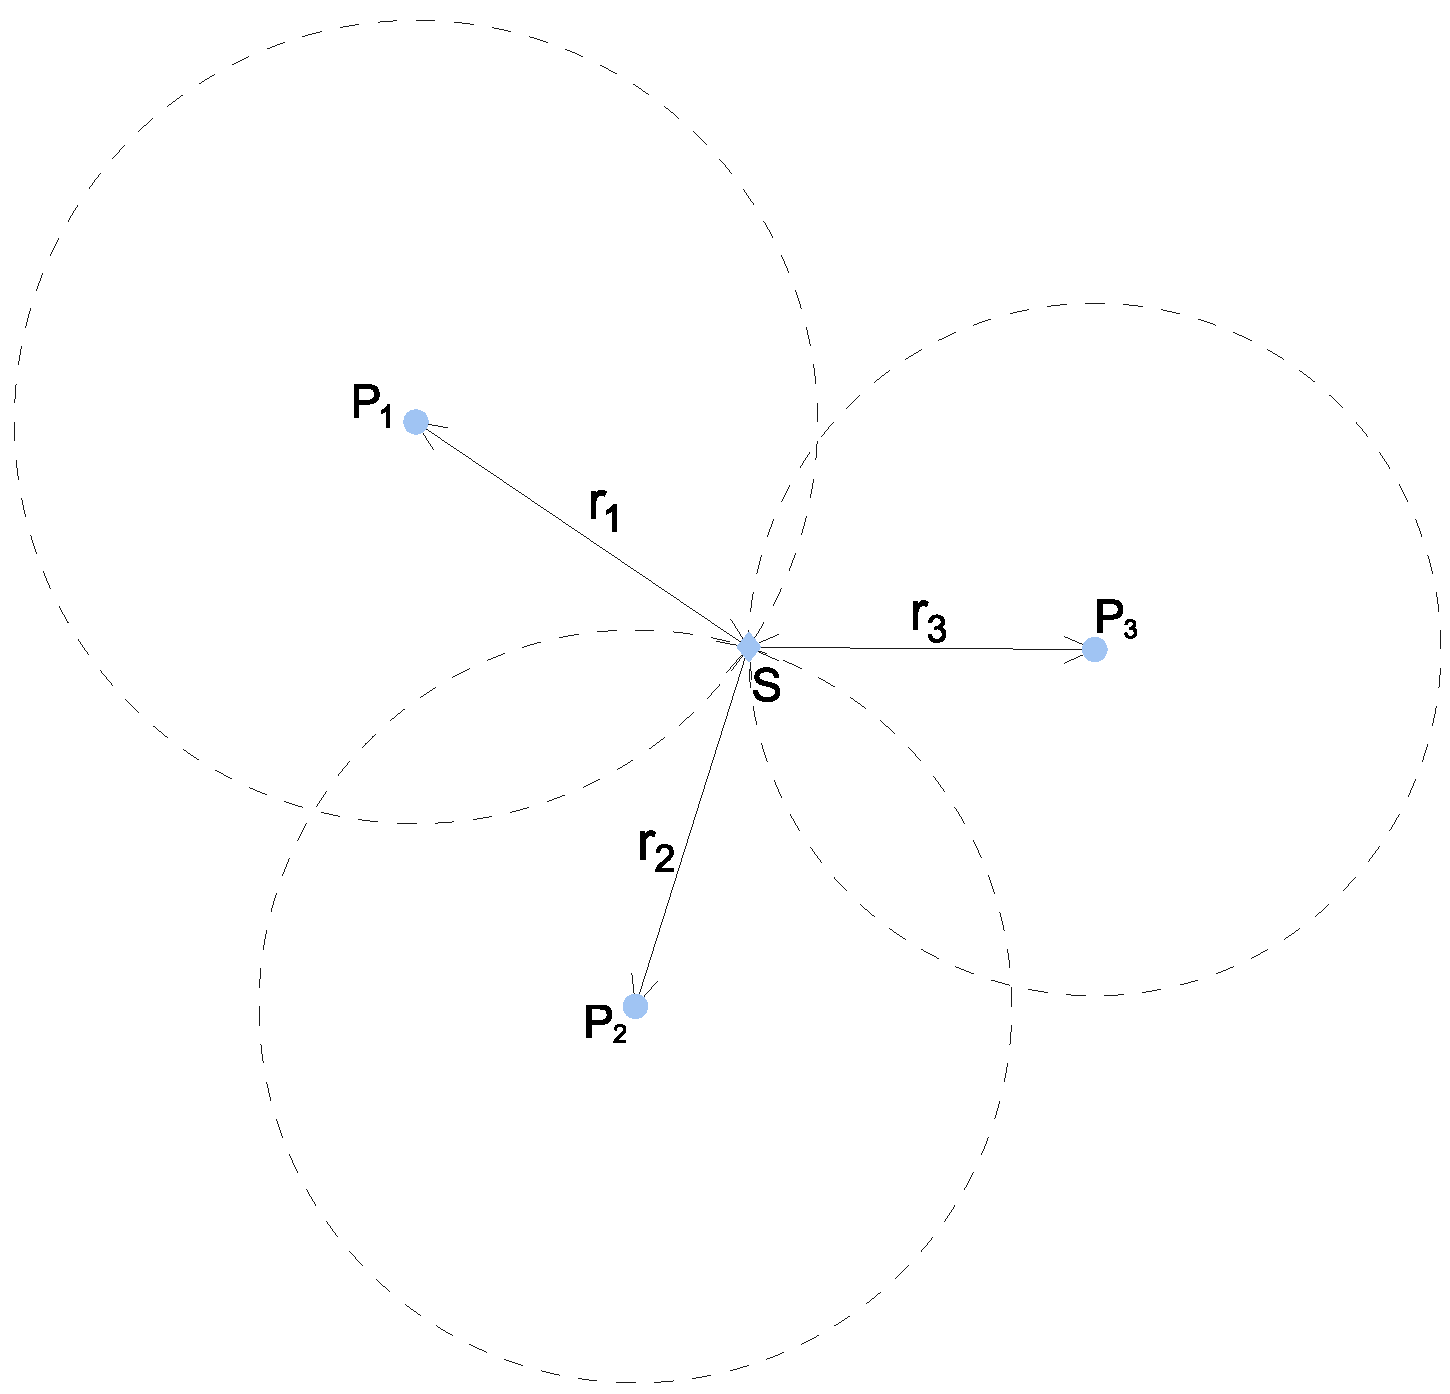
\includegraphics[width=0.6\textwidth]{toa.pdf}
        \caption{Posicionamiento 2D basado en la medida del ToA \cite{sayed.2005, Liu.2007}.}
        \label{fig:toa}
    \end{figure}
    
    Cabe destacar que para poder calcular la posición a través del tiempo de llegada, es necesario tener sincronía entre los emisores, pues es necesario conocer el tiempo inicial al transmitir. \\
    Además, en el contexto de los IPS, algunos de los problemas con ToA se agravan: primero, mientras que en GPS las posiciones de los satélites se conocen de antemano por sus parámetros orbitales, en IPS, este no es el caso, porque no hay una referencia general acordada. Segundo, para distancias muy cortas como las de interiores, las diferencias de tiempo serán extremadamente pequeñas para las señales de RF, por lo que se necesita una gran precisión.

    \subsection{Tiempo diferencial de llegada} \label{subsection:tdoa}
    La diferencia de tiempos de llegada (TDoA) se relaciona con la ToA porque utiliza el tiempo de viaje desde el transmisor al receptor para estimar las distancias, pero a veces el tiempo de emisión es desconocido. De esta forma, la diferencia de tiempos entre cada receptor es utilizada para estimar la distancia a cada uno de ellos. El cálculo de la diferencia de tiempos elimina la necesidad de conocer el tiempo de transmisión. Así pues, en métodos ToA o cualquier otro método basado en el tiempo, los dispositivos deben estar sincronizados para alcanzar medidas precisas. Sin embargo, como TDoA no utiliza la distancia entre transmisor y receptor, el transmisor no tiene porque estar sincronizado con el receptor. La sincronización solo se requiere entre todos los receptores, dado que la distancia se calcula gracias a la diferencia entre tiempo-distancia.
    
    \begin{figure}[h]
        \centering
        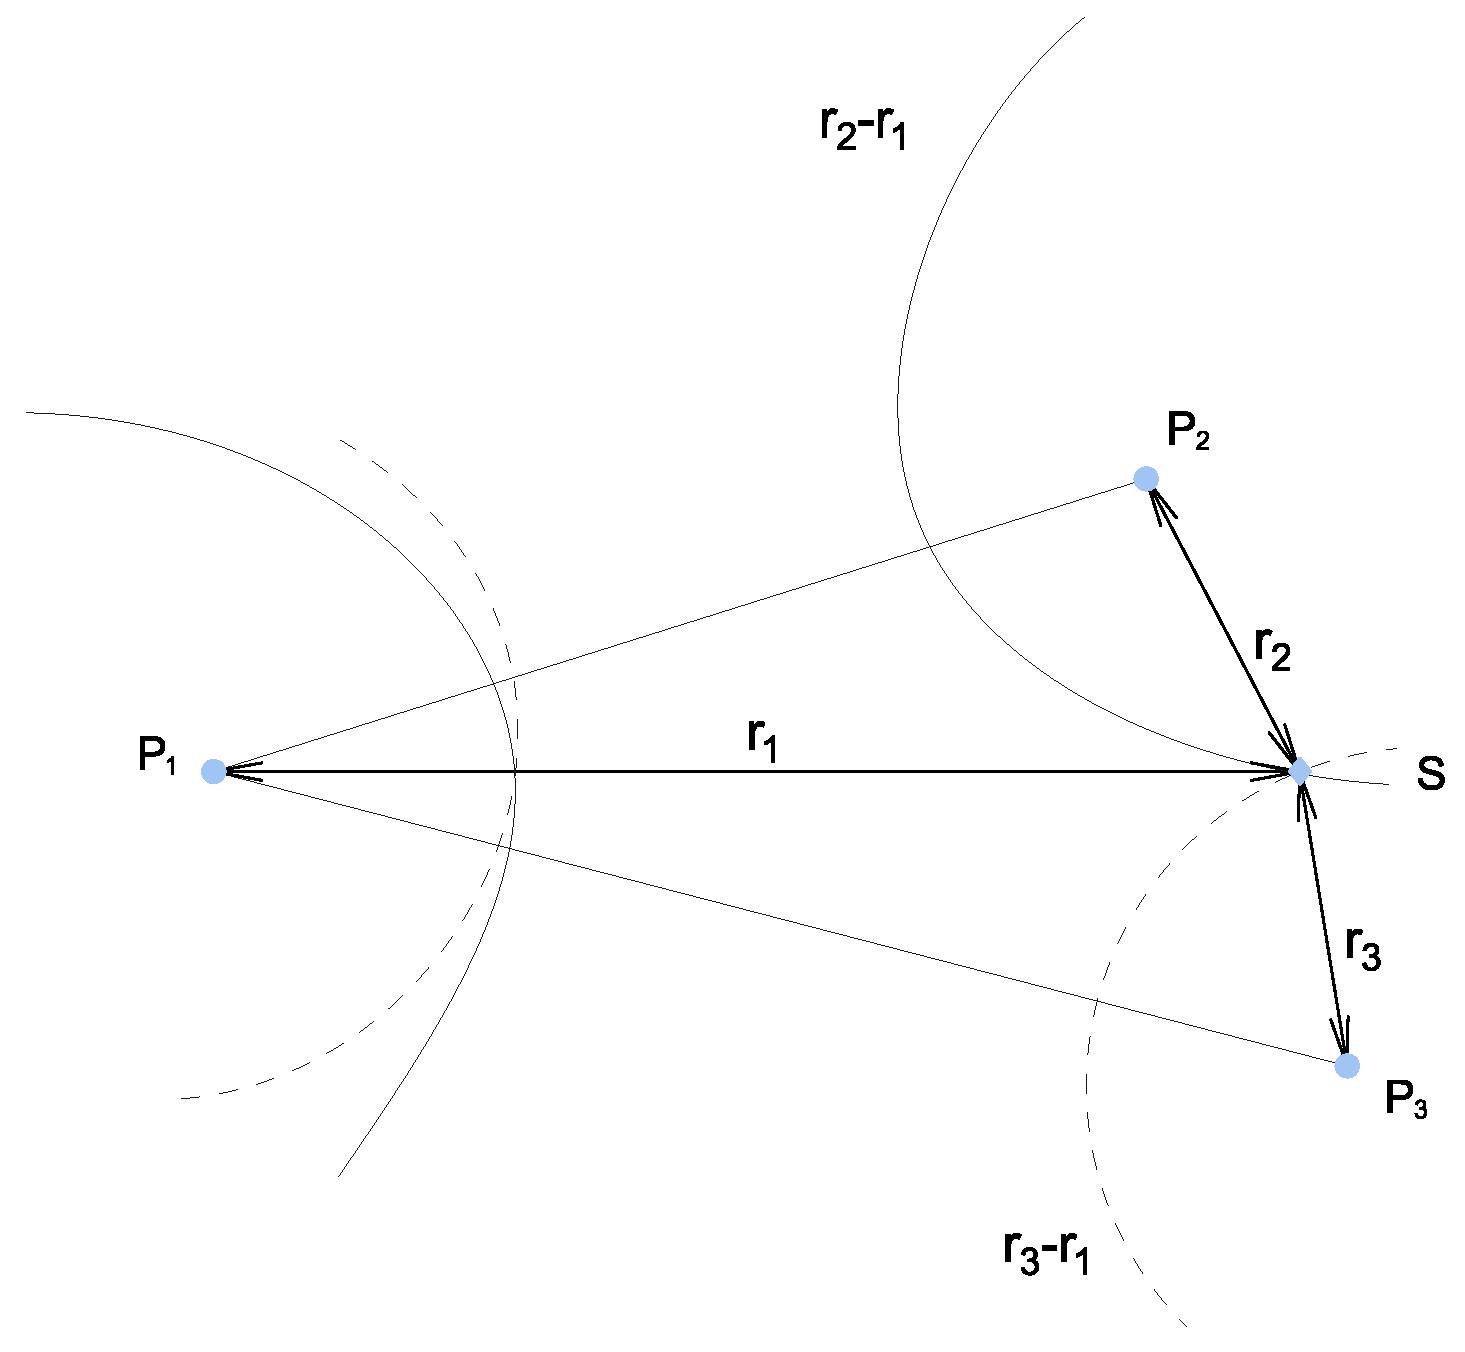
\includegraphics[width=0.6\textwidth]{tdoa.pdf}
        \caption{Posicionamiento 2D basado en la medida del TDoA \cite{sayed.2005, Liu.2007}.}
        \label{fig:tdoa}
    \end{figure}
    
    El posicionamiento en el plano de un objeto se puede estimar a partir de la intersección de dos o más mediciones de TDoA, como se muestra en la Figura \ref{fig:tdoa}. Dos hipérbolas se forman a partir de mediciones de TDoA en tres unidades de medición fijas ($P_1$, $P_2$ y $P_3$) para proporcionar un punto de intersección, que ubica el objeto $S$. \\
    De forma similar a como sucedía con el ToA en la Ecuación \ref{eq:rang_toa}, el rango de TDoA ($r_{i1}$) se puede calcular siguiendo la siguiente expresión:

    \begin{equation}
        r_{i1} = r_i - r_1 = c (t_i - t_1)
        \label{eq:rang_tdoa}
    \end{equation}

    \noindent donde $t_i - t_1$ es el TDoA asociado al punto $P_i$. En dos dimensiones, con $N$ referencias conocidas $P_1$, $P_2$, ... , $P_n$, con coordenadas cartesianas $(x_i, y_i)$, $i=1,...,n$, la posición $(\hat{x}, \hat{y})$ de un punto cualquiera $S$, se puede determinar utilizando los rangos $r_i$ \cite{sayed.2005}, calculados mediante la Ecuación \ref{eq:sist_tdoa}:
    
    \begin{equation}
        \begin{gathered}
            (r_{21} + r_1)^2 = x_2^2 + y_2^2 - 2 x_2 \hat{x} - 2 y_2 \hat{y} + r_1^2 \\
            (r_{31} + r_1)^2 = x_3^2 + y_3^2 - 2 x_3 \hat{x} - 2 y_3 \hat{y} + r_1^2 \\
            \vdots \\
            (r_{n1} + r_1)^2 = x_n^2 + y_n^2 - 2 x_n \hat{x} - 2 y_n \hat{y} + r_1^2 \\
        \end{gathered}
        \label{eq:sist_tdoa}
    \end{equation}
    
    Reorganizando términos, se obtiene:
    
    \begin{equation}
        \begin{gathered}
            - 2 x_2 \hat{x} - 2 y_2 \hat{y} = r_{21} r_1 + \frac{1}{2}(r_{21}^2 - x_2^2 - y_2^2) \\
            - 2 x_3 \hat{x} - 2 y_3 \hat{y} = r_{31} r_1 + \frac{1}{2}(r_{31}^2 - x_3^2 - y_3^2) \\
            \vdots \\
            - 2 x_n \hat{x} - 2 y_n \hat{y} = r_{n1} r_1 + \frac{1}{2}(r_{n1}^2 - x_n^2 - y_n^2) \\
        \end{gathered}
        \label{eq:sist_tdoa_2}
    \end{equation}
    
    y sabiendo que:
    
    \begin{equation}
        r_{1}^2 = \hat{x}^2 + \hat{y}^2
        \label{eq:rang_tdoa_2}
    \end{equation}
    
    En dos dimensiones para $N \geq 2$, el sistema de ecuaciones anterior está determinado, y resolviendo el mismo con la Ecuación \ref{eq:rang_tdoa_2} se podría hallar la posición del punto $S$ \cite{sayed.2005}. 
    
    Como una mejora en ToA, TDoA elimina la sincronización del transmisor para el tiempo de llegada y, por tanto, reduce su complejidad. Además, TDoA también proporciona una mejora en la precisión.

    \subsection{Intensidad de señal recibida} \label{subsection:rssi}
    La intensidad de la señal recibida (RSSI) es la intensidad de campo de una señal en el punto de recepción. RSSI se mide en el receptor, y con este dato la distancia puede ser estimada mediante modelos de propagación de la señal u otros métodos (ver Fig. \ref{fig:rssi}). En particular, modelos como la ecuación de propagación de Friis (Ec. \ref{eq:friis} \cite{friis.1946}) es utilizada con frecuencia \cite{goldoni.2010}. En otras ocasiones, modelos más complejos (Modelo de Propagación Elíptico \cite{zhou.2005}, EPM, o \emph{Fuzzy Inference System} \cite{teuber.2006}, FIS) son necesarios para determinar las pérdidas por propagación (PL, \emph{Path Loss}). 
    
    \begin{equation}
        P_R = P_T \dfrac{G_T G_R \lambda^2}{(4 \pi)^2 d^n}
        \label{eq:friis}
    \end{equation}
    
    Donde $P_R$ es la potencia de señal recibida o RSSI (en vatios, W), $P_T$ la potencia de señal transmitida (en vatios, W), $G_R$ la ganancia de antena recibida, $G_T$ la ganancia de antena transmitida, $\lambda$ la longitud de onda de la señal, la distancia $d$ (en metros, m) y la constante de propagación de Friis $n$. De esta ecuación, la distancia es fácilmente obtenible conociendo el resto de términos, que son fijos (salvo el RSSI) según la tecnología utilizada por el sistema.
    
    \begin{figure}[ht]
        \centering
        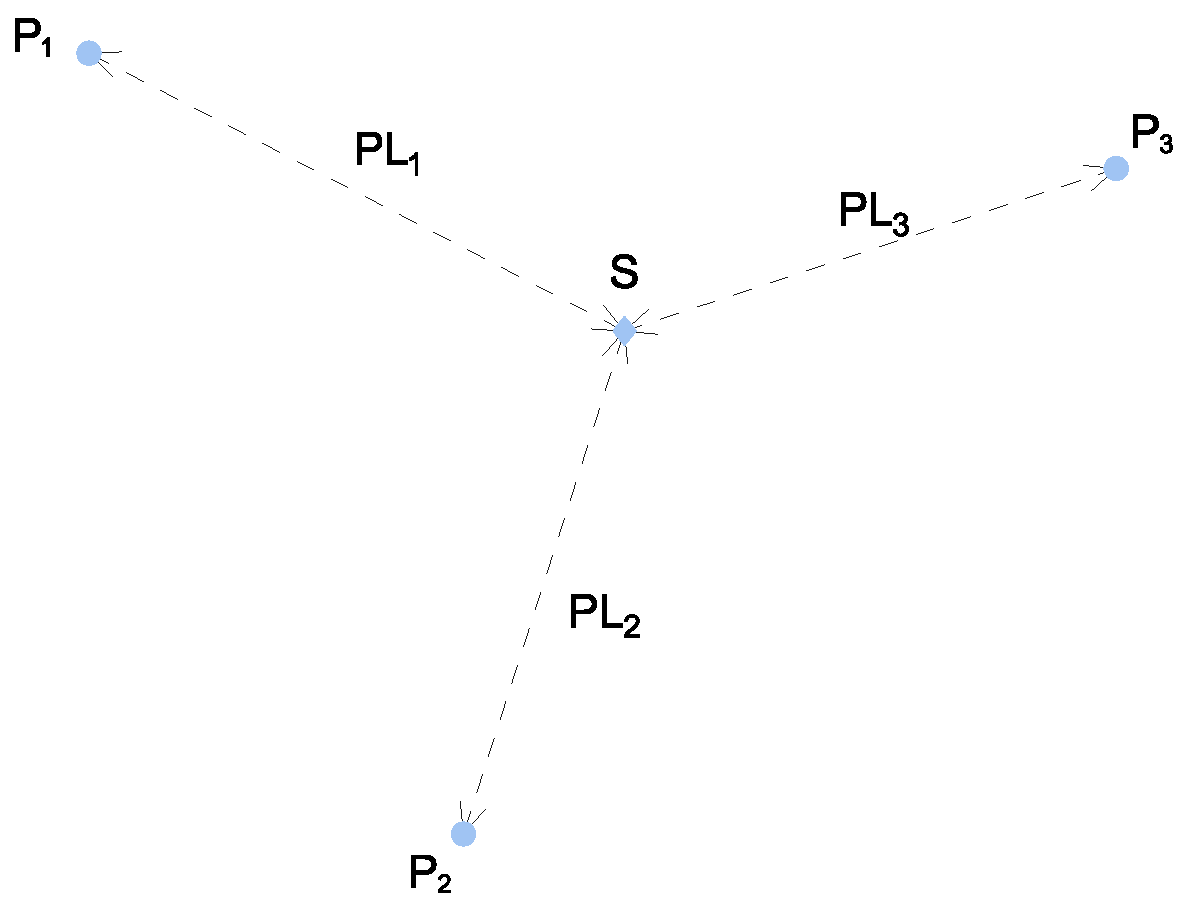
\includegraphics[width=0.6\textwidth]{rssi.pdf}
        \caption{Posicionamiento 2D mediante el calculo de la RSSI \cite{Liu.2007}.}
        \label{fig:rssi}
    \end{figure}
    
    Sin embargo, en entornos interiores donde es difícil obtener línea de visión directa (LoS), el RSSI y el posicionamiento pueden verse afectados por el multitrayecto y las oclusiones, lo que disminuye la precisión.
    
    Existen otras muchas métricas que no son descritas en este trabajo (RToF, PoA, PDoA, etc. \cite{Liu.2007}), pues la intención de este capítulo es introduir las técnicas más relevantes y utilizadas.
    
    \begin{table}[H]
    \centering
    \begin{threeparttable}
        \begin{tabular}{l l l l l}
            \toprule
            \thead{Propiedad} & \thead{Métrica} & \thead{Precisión} & \thead{Coste} & \thead{Complejidad} \\
            
            \midrule
            Directa & Distancia  & Alta  & Medio & Alta \\
            AoA     & Ángulo     & Alta\tnote{1}  & Alto & Alta \\
            ToA     & Distancia  & Alta  & Alto & Alta \\
            TDoA    & Distancia  & Alta  & Alto & Baja \\ 
            RSSI    & Atenuación & Media & Bajo & Baja \\
            \bottomrule
            \addlinespace[1ex]
        \end{tabular}
        
        \begin{tablenotes}\footnotesize
            \item[1] A pequeña escala (\emph{room level}). Para mayor cobertura la precisión decae.
        \end{tablenotes}
        
    \end{threeparttable}
    
    \caption{Resumen de las propiedades de la señal \cite{Sakpere.2017}.}
    \label{table:metrics}
    \end{table}

    
En resumen, las propiedades de la señal son un elemento importante para determinar la posición, ya que son necesarias en el cálculo y estimación de una posición. De estas propiedades dependen en parte parámetros importantes como la precisión, el coste o la complejidad del sistema resultante. En la Tabla \ref{table:metrics}, se resumen las características de las propiedades de la señal exploradas. \\ La propiedad de la señal utilizada con un algoritmo de posicionamiento determinará en gran medida la fuerza de la técnica de posicionamiento. Por ello, para usar la propiedad más apropiada, es importante entender los algoritmos de posicionamiento, que se presentan a continuación.


\section{Algoritmos de posicionamiento} \label{section:algoritmos}
Los algoritmos de posicionamiento cómo calcular la posición de un objeto. En otras palabras, estos algoritmos traducen las propiedades de la señal grabada en distancias y ángulos, y luego calculan la posición real de un objeto. Por ejemplo, cuando se estima la distancia entre un objeto y los puntos de referencia, el algoritmo calcula y determina la posición del objeto (ver Figura \ref{fig:integracion}). Tanto la propiedad de la señal como el algoritmo de posicionamiento trabajan juntos para determinar la posición de un objeto. El algoritmo de posicionamiento procesa la propiedad de la señal y genera una posición. \\
Los algoritmos de posicionamiento tienen ventajas y desventajas únicas, por lo que utilizar más de un tipo de algoritmo de posicionamiento al mismo tiempo mejorará la precisión y el rendimiento de la posición. Por lo tanto, existen varias métodos para determinar la posición utilizando información de orientación, rango o proximidad basada en la medición de señal. Las principales técnicas algorítmicas utilizadas en el posicionamiento son:

\begin{itemize}
    \item Multilateración.
    \item Análisis por proximidad.
    \item Análisis del entorno (\emph{fingerprinting}).
    \item Navegación por estima (navegación inercial, INS).
\end{itemize}

Las diversas propiedades de la señal se aplican dentro de los algoritmos de posicionamiento correspondientes.
 
    \subsection{Multilateración} \label{subsection:multilateracion}
    La multilateración utiliza la geometría para combinar las estimaciones de rango de diferentes dispositivos de referencia. Las estimaciones de rango podrían provenir de diferentes medidas, como RSSI, ToA, TDoA y AoA. Si se usan tres dispositivos de referencia en la combinación, entonces se llama trilateración o triangulación, en función de si se han utilizado distancias o ángulos. En concreto, estos métodos se han desarrollado en las Secciones \ref{subsection:aoa} AoA (triangulación) y \ref{subsection:toa} ToA (trilateración) al introducir las métricas de la señal.
    
    \subsection{Detección directa} \label{subsection:proximidad}
    Las técnicas por proximidad o detección directa consisten en determinar cuándo un objeto está ``cerca'' de una ubicación conocida, según lo registrado por un sensor dirigido específicamente a la detección por proximidad \cite{Hightower.2001}. Hay dos principales enfoques para detectar la proximidad: 
    
    \begin{itemize}
        \item Detectar un objeto con contacto físico a través de sensores táctiles, sensores de capacidad, y así sucesivamente, mediante medición directa.
        \item Detectar un objeto en un área de alcance de uno o más sistemas de identificación remota como Bluetooth o RFID, los cuales se introducirán más adelante (ver Fig. \ref{fig:proximidad}).
    \end{itemize}
    
    \begin{figure}[h]
        \centering
        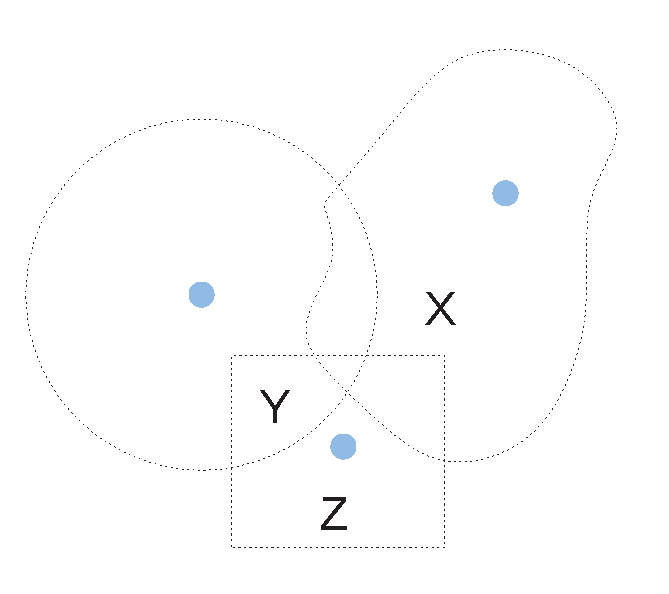
\includegraphics{photos/proximity.pdf}
        \caption{Esquema de detección por proximidad con sensores de diferente alcance \cite{Hightower.2001}.}
        \label{fig:proximidad}
    \end{figure}

    \subsection{Análisis del entorno} \label{subsection:fingerprinting}
    El \emph{fingerprinting} o análisis del entorno es un método utilizado para calcular ubicaciones aproximadas. El ``entorno'' puede ser de diferente naturaleza, desde cualquier fenómeno físico medible como señales Wi-Fi, Bluetooth o magnéticas, entre otras, hasta imágenes visuales capturadas con una cámara (Fig. \ref{fig:fingerprinting}). \\
    Se compone de dos fases: entrenamiento y determinación de posición. En la fase de entrenamiento, se graba un mapa de valores de intensidad de señal observados desde diferentes ubicaciones. Luego, en la fase de determinación de posición, los valores de intensidad de la señal observados en un dispositivo de usuario se comparan con los valores del mapa utilizando algoritmos de reconocimiento de patrones para inferir la ubicación actual del usuario. \\
    Los algoritmos más comunes son métodos probabilísticos \cite{kontkanen.2004}, \emph{$k$-nearest neighbor} ($k-NN$) \cite{jiang.2015}, redes neuronales \cite{battiti.2002}, máquinas de vectores de soporte (SVM, \emph{Support Vector Machine}) \cite{brunato.2005}, \cite{wu.2004} y polígono de M-vértices más pequeño (SMP, \emph{smallest M-vertex polygon}) \cite{prasithsangaree.2002}.
   
    \begin{figure}[h]
        \centering
        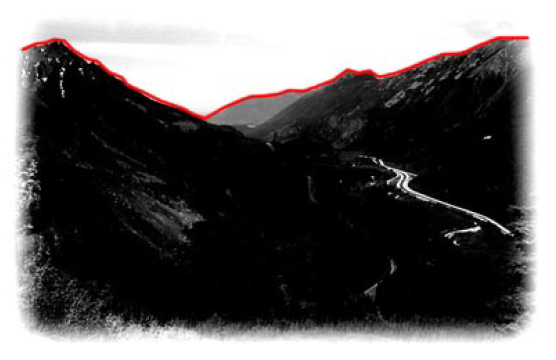
\includegraphics[width=0.7\textwidth]{photos/scene_analysis.PNG}
        \caption{Análisis de una imagen visual como técnica \emph{fingerprinting} \cite{Hightower.2001}.}
        \label{fig:fingerprinting}
    \end{figure}
   
    Por último, es importante mencionar una técnica ampliamente utilizada en robótica conocida como localización y mapeo simultáneo (SLAM, \emph{Simultaneous Localization and Mapping}) \cite{dissanayake.2001}, \cite{cadena.2016}. SLAM comprende la capacidad de colocar un vehículo autónomo en una ubicación desconocida con un entorno desconocido, la construcción de un modelo (el mapa) utilizando solo las observaciones relativas del entorno, y el uso este mapa simultáneamente para navegar. \\
    La necesidad de utilizar un mapa del entorno es doble. Primero, el mapa a menudo se requiere para soportar otras tareas; por ejemplo, un mapa puede informar la planificación de la ruta o proporcionar una visualización intuitiva para un operador humano. En segundo lugar, el mapa permite limitar el error cometido al estimar el estado del robot;por ejemplo, el robot puede ``restablecer'' su error de localización al volver a visitar áreas conocidas. \\
    La principal ventaja de SLAM es que elimina la necesidad de infraestructuras artificiales o un conocimiento topológico del entorno a priori. Una solución al problema de SLAM sería de un valor inestimable en una gama de aplicaciones en las que no se puede obtener una posición absoluta o información precisa del mapa, incluidos, entre otros, la exploración planetaria autónoma, los vehículos submarinos autónomos, los vehículos autónomos aéreos y los todoterreno autónomos.
   
    \subsection{Navegación por estima} \label{subsection:estima}
    La estimación de una posición futura dada una inicial y una velocidad y dirección es, de hecho, uno de los métodos más antiguos para la navegación, a menudo llamado \emph{dead reckoning} o navegación inercial. Un problema obvio con la navegación por estima es la acumulación progresiva de errores, ya que un pequeño error en la dirección podría significar un gran error a medida que se viaja una gran distancia. \\
    En los sistemas modernos, los métodos inerciales utilizan acelerómetros y giróscopos y, en general, combinan su información con otros sensores para lograr un buen rendimiento. Los acelerómetros se pueden usar para determinar las modificaciones en la posición del objeto cuando se detecta una aceleración en una dirección determinada. Por supuesto, esta es una estimación muy aproximada, que puede mejorarse utilizando un giróscopo para cambios de dirección. \\
    
    En la Tabla \ref{table:algorit} se resumen las características principales de los algoritmos presentados previamente.
    
    \begin{table}[H]
    \centering
    \begin{threeparttable}

        \begin{tabular}{l l l l l l l} 
            \toprule
            \thead{Algoritmo} & \thead{Propiedad} & \thead{Precisión} & \thead{Coste} & \thead{Complejidad} & \thead{Otros} \\
            \midrule
            Triangulación & AoA      & Alta\tnote{a} & Bajo & Baja & \\ 
            Trilateración & ToA/TDoA & Alta  & Alto & Alta & Sincronización \\
                          &          &       &      &      & requerida \\
            Detección     & RSSI     & Alta  & Alto & Alta & Alta densidad \\
            directa       &          &       &      &      & de readers \\
            Análisis del  & RSSI     & Media & Alto & Alta & Alto rendimiento \\
            entorno       &          &       &      &      & y baja velocidad \\
            Navegación    & -        & Alto  & Bajo & Baja & Sensible a \\
            por estima    &          &       &      &      & errores \\
            \bottomrule
        \end{tabular}
    
        \begin{tablenotes}\footnotesize
            \item[a] A pequeña escala (\emph{room level}). Baja precisión, alto coste y alta complejidad según ampliamos el área de cobertura.
        \end{tablenotes}
    \end{threeparttable}
    
    \caption{Resumen de los algoritmos de posicionamiento \cite{Sakpere.2017}.}
    \label{table:algorit}
    \end{table}